\documentclass[11pt]{article}
\usepackage{deauthor,times,graphicx}
\usepackage{authblk}
\usepackage{amsfonts}
\usepackage{tikz}
\usetikzlibrary{shapes, arrows, positioning}
\usepackage{amsmath}
\usepackage{amssymb}
\usepackage{bm}

\usepackage{graphicx}
\usepackage{algorithm2e}
\usepackage{subcaption}

\newcommand{\classifier}{\ensuremath{h}}
\newcommand{\Dom}[1]{\textsc{Dom}(#1)}

\newcommand{\popul}{\Delta}
\newcommand{\targetpopul}{\mathcal{D}^*}
\newcommand{\underlyingDist}{\Omega}
\newcommand{\protectedAttr}{s}
\newcommand{\protG}{s_0}
\newcommand{\privG}{s_1}
\newcommand{\ProtectedAttr}{S}

\newcommand{\repairs}{\ensuremath{\mathsf{Repairs}}\xspace}
\newcommand{\GAPair}{\mathcal{I}_{\underlyingDist}}
\newcommand{\auxdata}{\mathcal{A}_{\underlyingDist}}
\newcommand{\lowerbound}{{\text{CLB}}}
\newcommand{\upperbound}{\text{CUB}}
\newcommand{\NPos}[1]{\texttt{N}_{#1}^{+}}
\newcommand{\cdag}{G}
\newcommand{\bcdag}{\mathcal{G}}
\newcommand{\bdata}{D_{\popul}}
\newcommand{\dtrain}{\bdata^{tr}}
\newcommand{\dtest}{D_{\underlyingDist}^{ts}}
\newcommand{\bdtrain}{D^{c}_{tr}}
\newcommand{\admis}{\boldsymbol{a}}
\newcommand{\Admis}{\boldsymbol{A}}
\newcommand{\dist}{{\underlyingDist}}
\newcommand{\eCondDemoParityDist}[2]{\hat{\digamma}_{\classifier, {#1}}(#2)}
\newcommand{\seCondDemoParityDist}[1]{\hat{\digamma}(#1)}
\newcommand{\CondDemoParityDist}[2]{\digamma_{\classifier, {#1}}(#2)}
\newcommand{\sCondDemoParityDist}[1]{\digamma(#1)}
\newcommand{\CondDemoParity}[1]{\digamma_{\classifier, {#1}}(\underlyingDist)}
\newcommand{\CondDemoParityb}[1]{\digamma_{\classifier, {#1}}(\popul)}
\newcommand{\sCondDemoParity}{\digamma(\underlyingDist)}
\newcommand{\sCondDemoParityb}{\digamma(\popul)}
\newcommand{\Pa}{\boldsymbol{Pa}}
\newcommand{\pr}{{\tt \mathrm{Pr}}}

\newcommand{\babak}[1]{{\texttt{\color{red} Babak: [{#1}]}}}
\newcommand{\red}[1]{{\color{red} [{#1}]}}
% \newcommand{\red}[1]{{#1}}
\newcommand{\jiongli}[1]{{\texttt{\color{magenta} Jiongli: [{#1}]}}}
\newcommand{\nindep}{\mbox{$\not\!\perp\!\!\!\perp$}}
\newcommand{\indep}{\mbox{$\perp\!\!\!\perp$}}

\newcommand{\crab}{\textsc{Crab}\xspace}
\newcommand{\capuchin}{\textsc{Capuchin}\xspace}
\newcommand{\groundtruth}{Unbiased Data\xspace}
\newcommand{\training}{Biased Data\xspace}
\newcommand{\ipw}{IPW\xspace}
\newcommand{\crabphi}{\crab (w/o External)}
\newcommand{\crabsuff}{\crab (w/ External)}
\newcommand{\clbphi}{\textsc{CLB}-$\emptyset$\xspace}
\newcommand{\cubphi}{\textsc{CUB}-$\emptyset$\xspace}
\newcommand{\clbsuff}{\textsc{CLB}-\textsc{SUFF}\xspace}
\newcommand{\cubsuff}{\textsc{CUB}-\textsc{SUFF}\xspace}




\begin{document}

\title{Overcoming Data Biases: Towards Enhanced Accuracy and Reliability in Machine Learning}
\author{Jiongli Zhu, Babak Salimi\\
University of California San Diego\\
\{jiz143, bsalimi\}@ucsd.edu}

\maketitle

\begin{abstract}

The pervasive integration of machine learning (ML) across various sectors has underscored the critical challenge of addressing inherent biases in ML models. These biases not only undermine the models' fairness and accuracy but also have significant real-world consequences. Traditional approaches to mitigating these biases often fail to address their root causes, leading to solutions that may superficially seem fair but do not tackle the underlying problems. This review paper explores the role of causal modeling in enhancing data cleaning, preparation, and quality management for ML. By analyzing existing research, we demonstrate how causal reasoning can effectively identify and rectify data biases, thus improving the fairness and accuracy of ML models. We advocate for the increased adoption of causal approaches in these processes, emphasizing their potential to significantly enhance the integrity and reliability of data-driven technologies.

\end{abstract}


%%%%%%%% intro %%%%%%%%
\section{Introduction}

Machine Learning has become integral to sectors such as healthcare, finance, and law enforcement, spotlighting the importance of addressing biases and inaccuracies in ML models. These critical issues necessitate the development of ML models that are reliable, accurate, and fair, given their significant impact on individuals and communities. Consequently, substantial research efforts have been dedicated to mitigating algorithmic bias, aiming to enhance the robustness, reliability, accuracy, and fairness of ML models~\cite{mehrabi2021survey,balayn2021managing}.

Despite numerous efforts to address data biases in ML, current strategies often focus on alleviating the symptoms rather than confronting the underlying causes of these biases. This approach may inadvertently lead to ``fair-washing," where superficial measures worsen the problems they intend to solve~\cite{zhu2023consistent}. In the realm of developing fair ML models, prevalent methods include: (1) integrating fairness metrics into the optimization process during training, known as in-processing~\cite{calders2010three,zhang2021omnifair,zhang2018mitigating,kearns,celis2019classification,kamishima2012fairness}, and adjusting the model’s output post-training, referred to as post-processing~\cite{pmlr-v65-woodworth17a,pleiss2017fairness,hardt2016equality,kamiran2012decision}; and (2) modifying the data before training, or pre-processing, to achieve a more balanced distribution~\cite{zemel2013learning,galhotra2022causal,salimi2019capuchin,calmon2017optimized,kamiran2012data}. However, these approaches often operate under the assumption that the training data is representative of the actual distribution~\cite{islam2022through}, a premise that is frequently flawed. Data biases, such as confounding, measurement, and selection biases, along with other data quality issues, distort the data distribution~\cite{neutatz2021cleaning, zhu2023consistent, mehrabi2021survey, chakraborty2021bias, olteanu2019social, gianfrancesco2018potential}, often leading to training datasets that do not accurately represent the target population. This mismatch poses challenges in preprocessing the data to obtain a representative sample. Consequently, ML models trained with such biased data are likely to underperform, being unfair and inaccurate when applied to the target population and during the inference process.


Considerable efforts have been directed toward mitigating data biases, including selection bias~\cite{huang2006correcting,cortes2008sample,liu2014robust,rezaei2020robust,du2021robust} and labeling errors~\cite{jiang2020identifying,zhang2023mitigating,zhang2023iflipper}. Yet, these initiatives often hinge on significant assumptions—like the presence of an unbiased sample or specific presumptions regarding data quality issues—that are challenging to verify in real-world settings. Such reliance introduces complications, rendering these strategies less effective for practical applications. Furthermore, traditional data cleaning techniques~\cite{mahdavi2020baran,DBLP:journals/pvldb/RekatsinasCIR17,krishnan2016activeclean,DBLP:journals/pvldb/KarlasLWGC0020} may falter in restoring the ground truth or in ensuring datasets accurately reflect their target domains. Occasionally, it may be inherently unfeasible to obtain a representative sample to efficiently counter data biases. Overlooking these pivotal concerns may inadvertently perpetuate existing biases within the data~\cite{schelter2021jenga,guhaautomated,neutatz2021cleaning}.


In this paper, we explore data biases through a causal lens, integrating concepts from  ML , causal inference, and data management. Our primary objective is to highlight the significant potential of causal reasoning in enhancing data cleaning techniques, with a particular focus on data quality management research. Causal reasoning facilitates a more thorough examination and validation of the assumptions underlying data collection processes and data provenance, thereby increasing transparency. By reviewing recent studies that employ causal inference for debiasing data, we aim to showcase the considerable impact of this methodology. Our analysis focuses on incorporating causal methods into existing frameworks for data quality management and cleaning, with the goal of reducing biases and improving both the fairness and accuracy of ML models. This specific investigation contributes to the expanding field of data quality management research, an essential component of data management. We advocate for ongoing research and development aimed at forging more robust, unbiased, and effective data-driven technologies, achieved through the refinement of data management practices.




%%%%%%%% data biases %%%%%%%%
\vspace{-.4cm}
\section{Data Biases}
\vspace{-.2cm}

{\em Data bias} refers to systematic errors within datasets that lead to outcomes that are either inaccurate, unfair, or unreliable. These biases often manifest as uncertainties and incompleteness in data and systematic deviations in the data distribution, compromising its representation of the actual phenomena under study. In the context of knowledge extraction, these biases can lead to analyses that yield incorrect conclusions and false discoveries. In the context of ML, if these biases are not adequately addressed, they can be learned and perpetuated by downstream models, impacting their accuracy and fairness. In this section, we explore the most common sources of data bias in real-world applications, with a specific focus on challenges such as bias due to missing data, confounding variables, and erroneous measurements~\cite{zhioua2023dissecting,goel2021importance,bareinboim2012controlling,pearl2012measurement,mehrabi2021survey}. Understanding and addressing these factors is vital for assessing the quality and reliability of data used in ML.


\vspace{-0.4cm}
\paragraph{Bias due to Missing Data:} During data collection, certain portions of data may be missing for various reasons, such as high data collection costs for specific sub-populations or historical discrimination~\cite{antman1985selection}. This missing data can manifest as either \textit{missing values within tuples} or \textit{entirely missing tuples}. It is particularly challenging when entire tuples are missing non-randomly, leading to {\em selection bias}~\cite{choi1995effect}. This bias occurs when the data collection process or the selection of training data is influenced by specific attributes, resulting in a subset that does not accurately represent the entire population. Even in scenarios where recovery is theoretically possible~\footnote{Recoverability of a distribution from missing data, biases, or data quality issues, in principle, refers to the capacity to accurately and consistently (asymptotically) estimate the underlying probability distribution or statistical properties of a dataset, even in the presence of such data quality challenges.}, 
such as cases of data missing completely at random or when an unbiased sample is available, the existing approaches for dealing with missing data imputation or selection bias typically only provide asymptotic guarantees~\cite{rubin1978multiple,schenker1988asymptotic,kim2004finite}. In practical applications with finite data, these methods might display unpredictable behavior and still lead to biased samples. The non-random nature of missing data thus presents significant challenges in obtaining unbiased data that accurately reflects the underlying distribution, highlighting a crucial concern in data management and ML. We illustrate with two examples: 


\begin{example}[Missing Attribute Values]\label{ex:missing-val-children-health}
Missing data presents a formidable challenge in critical areas such as healthcare and finance, characterized by its non-random occurrence and complex mechanisms. In pediatric health studies, for example, in cancer research, parents' hesitancy to divulge sensitive prognosis details, like life expectancy, results in crucial information being omitted. Studies have shown that such omissions correlate with poorer survival outcomes in comprehensive cancer registries~\cite{Rosenberg2014What's, plichta2023implications}. Similarly, financial ML applications face missing data, particularly in loan application datasets, where information on repayment potential for rejected applicants or those with restricted financial access is often absent. This gap, largely due to historical and racial biases, distorts data distribution. If not addressed, this distortion leads to inaccurate estimations and perpetuates biases in these sectors~\cite{plichta2023implications,luo2017validity,ehrhardt2021reject}.
\end{example}

\vspace{-.2cm}
\begin{example}[Selection Bias]\label{ex:selection-bias-sensitive-domains}
Selection bias is prevalent in many sensitive domains, such as health care, finance, and predictive policing.
In predictive policing, selection bias may occur when historical crime data, which often reflects past law enforcement and societal biases, is used to train ML models. This can lead to a cycle where certain communities are over-policed based on biased data, further perpetuating the bias in future decision makings~\cite{brayne2015predictive,lum2016predict}. 
In covid-19 studies, selection bias can arise when the data is collected from a population of individuals who are hospitalized or have tested positive, leading to a false association between the test positive rate and ethnic minorities due to barriers in healthcare access~\cite{griffith2020collider}.
In finance, selection bias can manifest in credit scoring where historical lending data may disproportionately represent certain socio-economic groups, such as individuals from higher income areas. This can lead to unfair or inaccurate credit decisions when the model is applied to populations from diverse economic backgrounds, including underdeveloped regions~\cite{banasik2003sample, verstraeten2005impact}. 
\end{example}

\vspace{-.3cm}
\paragraph{Bias due to Latent Confounding:} Confounding bias arises in ML when unobserved confounders affect both predictors and outcomes, leading to spurious correlations and misinterpreted causal relationships~\cite{pearl2009causality}. This bias can distort conclusions, making data associations that seem causal when they are not. In ML, models trained on such data may base predictions on these unreliable correlations, resulting in inaccuracies and poor generalization across real-world scenarios~\cite{arjovsky2019invariant,yarkoni2022generalizability,hu2022improving}.

\vspace{-.1cm}
\begin{example}[Confounding Bias]\label{ex:confounding}
Confounding bias significantly impacts ML applications in healthcare and social media analytics. In healthcare, for instance, ML models trained on skin cancer images may falsely associate surgical markings with disease severity, misguiding the diagnosis~\cite{winkler2019association,esteva2017dermatologist}. Similarly, pneumonia detection models may inaccurately correlate device fingerprints with the disease by using data pooled from hospitals with varying pneumonia rates, leading to misidentifications based on hospital systems rather than the disease itself~\cite{zech2018variable}. In social media analytics, complex relationships between various factors and self-harm tendencies create biased associations between social media use and self-harm, complicating the analysis~\cite{tormoen2023nationwide}.
\end{example}

\vspace{-.3cm}
\paragraph{Bias due to Measurement Error:} 
Measurement errors arise when there is a discrepancy between the true value of a variable and the value obtained through measurement or observation. When these errors are not random but systematically affect certain sub-populations, this results in skewed data distribution, a situation known as measurement bias~\cite{pearl2012measurement,kuroki2014measurement,millsap1993methodology}.
A prevalent form of measurement bias is label bias. Label bias arises when irrelevant factors, such as sensitive demographic information, influence the assigned labels during the data collection process.

\begin{example}[Measurement Bias]
In epidemiological studies estimating cardiovascular risk from dietary habits, reliance on self-reported dietary intake questionnaires can introduce measurement bias. Participants often misreport consumption—understating unhealthy and overstating healthy foods due to social desirability—skewing data away from true dietary patterns. This misalignment can lead models to underestimate the benefits of healthy diets on heart disease prevention~\cite{Page2008Appraising}. Similarly, in computer vision or natural language processing, crowdsourced data labeling can embed label bias. For example, facial recognition models may perform poorly on certain ethnic groups if labels are influenced by unconscious stereotypes, undermining the model's accuracy and fairness in applications like surveillance~\cite{haliburton2023investigating}.
\end{example}

%%%%%%%% causal modeling %%%%%%%%

\section{Causal Modeling of Data Biases}\label{section:causalmodeling}

In this section, we demonstrate the essential role of causal modeling in addressing various data biases. Causal modeling provides a structured framework for understanding and capturing the provenance of data collection processes, along with their intricacies. This approach is crucial in identifying the sources of bias and plays a key role in informing the development and implementation of data debiasing and cleaning algorithms. By leveraging causal relationships, these algorithms are better equipped to tackle the root causes of bias, rather than merely addressing their symptoms. Such an approach leads to the creation of a more robust and reliable dataset, which is vital for building fair and accurate ML models.
\vspace{-.3cm}
\paragraph{Causal Diagrams:} A causal diagram or causal graph is a directed graph that represents the causal relationships between a collection of observed or unobserved (latent) variables and models the underlying process that generates the observed data. Each node in a causal diagram corresponds to a variable, and an edge between two nodes indicates a potential causal relationship between the two variables.  To illustrate, consider the causal diagram shown in Figure~\ref{fig:selection-bias}. In this graph, the edge from the various factors such as education and income ($\boldsymbol{W}$) to the crime risk ($Y$) indicates that these factors of a person causally influence their risk of committing crimes. 

\vspace{-.3cm}
\paragraph{$d$-separation and Conditional Independence:} Causal diagrams encode a set of conditional independences that can be read off the graph using $d$-separation~\cite{pearl2009causality}. 
Two nodes are $d$-separated by a set of variables $\bm{V}_m$ in causal diagram $G$, denoted $(V_l \indep V_r \mid_d \bm{V}_m)$ if for every path between them, one of the following conditions holds:
(1) the path contains a {\em chain} ($V_l \rightarrow V \rightarrow V_r)$  or a {\em fork} ($V_l \leftarrow V \rightarrow V_r)$ such that $V \in \bm{V}_m$, and (2) the path contains a {\em collider} ($V_l \rightarrow V \leftarrow V_r)$ such that $V  \not\in \bm{V}_m$,  and no descendants of $V$ are in $\bm{V}_m$. 
A distribution is said to be {\em Markov compatible} with a causal graph if \( d \)-separation within the graph implies conditional independence in the data distribution, i.e., \( (V_l \indep V_r \mid_d \bm{V}_m) \Rightarrow (V_l \indep V_r \mid \bm{V}_m) \). 
Continuing with the causal diagram in Figure~\ref{fig:selection-bias}, the graph encodes the \( d \)-separation statement \( (Y \indep \ \text{Zip} \mid_d \boldsymbol{W}) \).
For any distribution that is Markov compatible with this graph, this \( d \)-separation implies that crime risk (\( Y \)) and neighborhood (\( \text{Zip} \)) are independent, conditioned on education and income (\( \boldsymbol{W} \)). 
In this paper, assuming Markov compatibility, we consider \( d \)-separation to always imply conditional independence and use these terms interchangeably.


Next, we model each of the data biases using causal diagrams. Our discussion primarily centers on three specific types of biases: non-random missing values and selection bias as instances of bias due to missing data, confounding bias resulting from variable omission, and label bias as a manifestation of measurement errors.
In addition, we explore existing research that addresses various forms of data biases in ML applications and discuss recent works that utilize the conditional independences encoded in causal diagrams for building fair ML models. 
\vspace{-.3cm}
\paragraph{Algorithmic Fairness:}
Fairness in  ML centers around a model $\classifier$ producing an output $h(\boldsymbol{x})$ and considering a protected attribute $\ProtectedAttr$, like gender or race. Many existing definitions of fairness require some form of statistical independence between the model's output and the protected attribute, which is sometimes conditioned on a third set of variables~\cite{mehrabi2021survey}. For instance, \textit{statistical parity} (\cite{dwork2012fairness}) necessitates equal positive and negative prediction rates across different groups, formalized as $(\ProtectedAttr \indep h(\boldsymbol{x}))$. \textit{Equalized odds} (\cite{hardt2016equality}) aims for parity in false positive and negative rates across groups, denoted as $\mbox{$(\ProtectedAttr \indep h(\boldsymbol{x}) \mid Y)$}$. 
Meanwhile, \textit{conditional statistical parity} seeks consistent positive classification probabilities across groups when accounting for certain permissible attributes $\Admis$, which are considered non-discriminatory factors in decision-making, expressed as $\mbox{$(\ProtectedAttr \indep h(\boldsymbol{x}) \mid \Admis)$}$. Notably, conditional statistical parity is a more general fairness concept compared to the others. When the set of admissible features $\Admis$ is empty, it simplifies to statistical parity, and when $\Admis$ includes the outcome label $Y$, it becomes equivalent to equalized odds. Many other associational and causal fairness criteria can also be expressed as conditional independence constraints~\cite{salimi2020database}.


\begin{figure}[t]
\centering
\begin{subfigure}[b]{0.24\textwidth}
   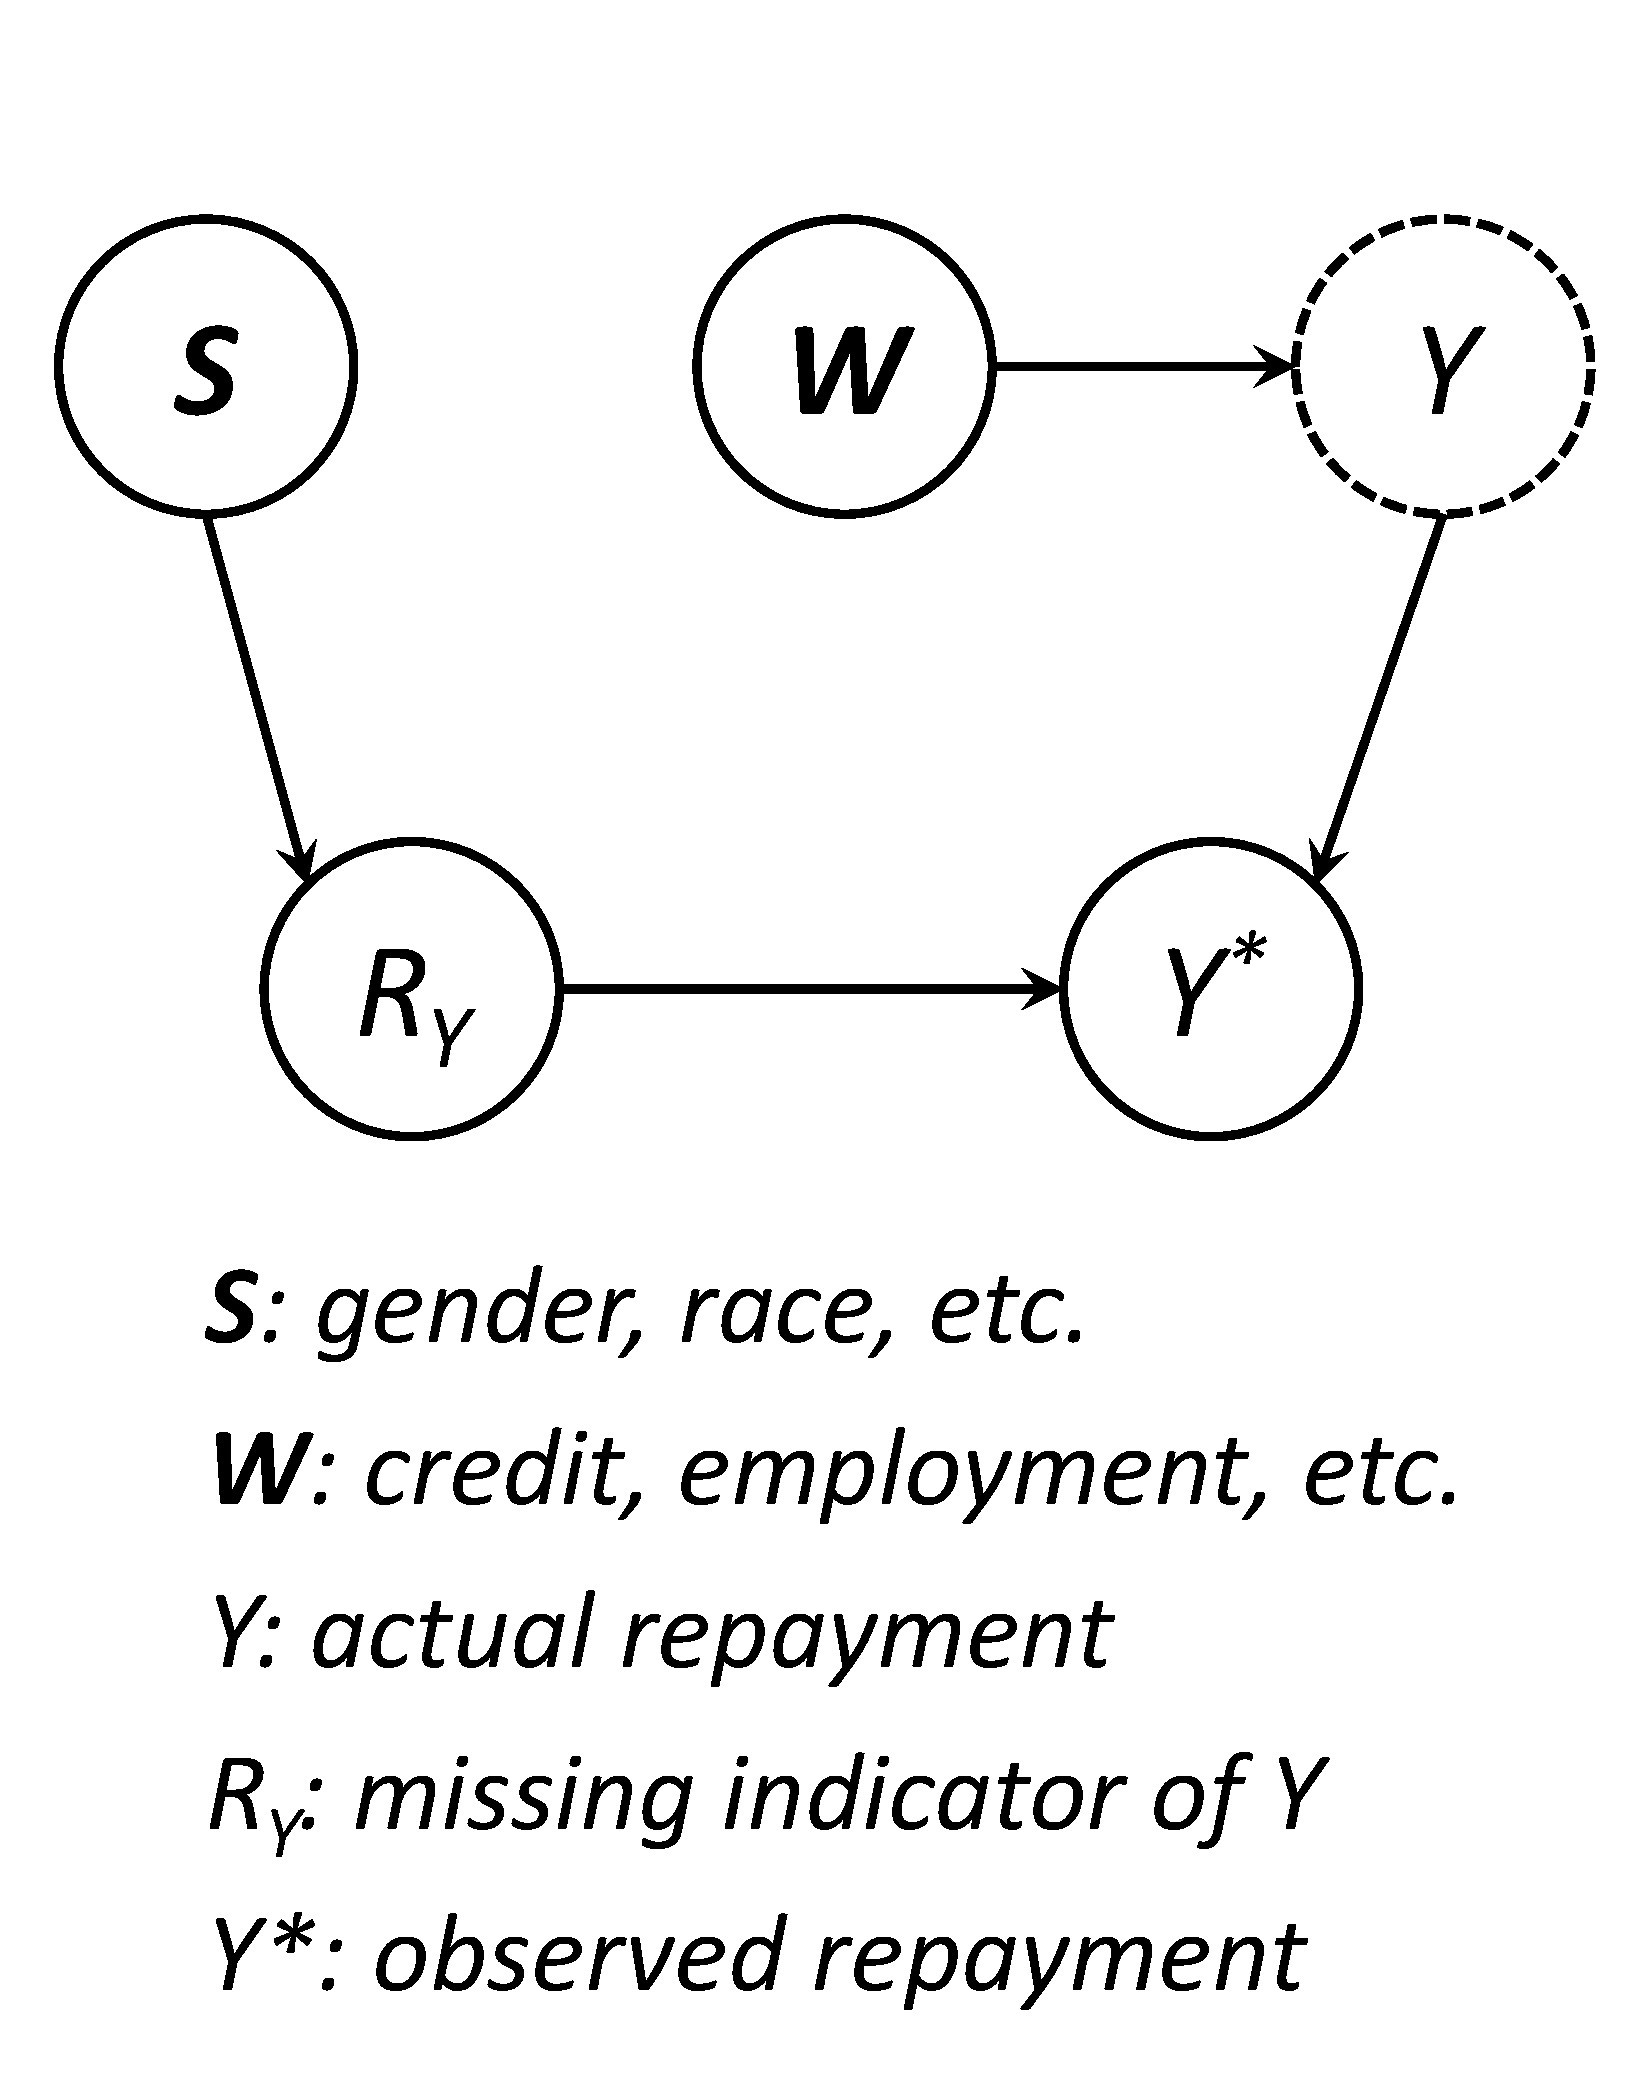
\includegraphics[width=\linewidth]{submissions/submission5/figs/missing-value.pdf}
   \vspace{-.5cm}
   \caption{}
   \label{fig:missing-value}
\end{subfigure}
\hfill
\begin{subfigure}[b]{0.24\textwidth}
   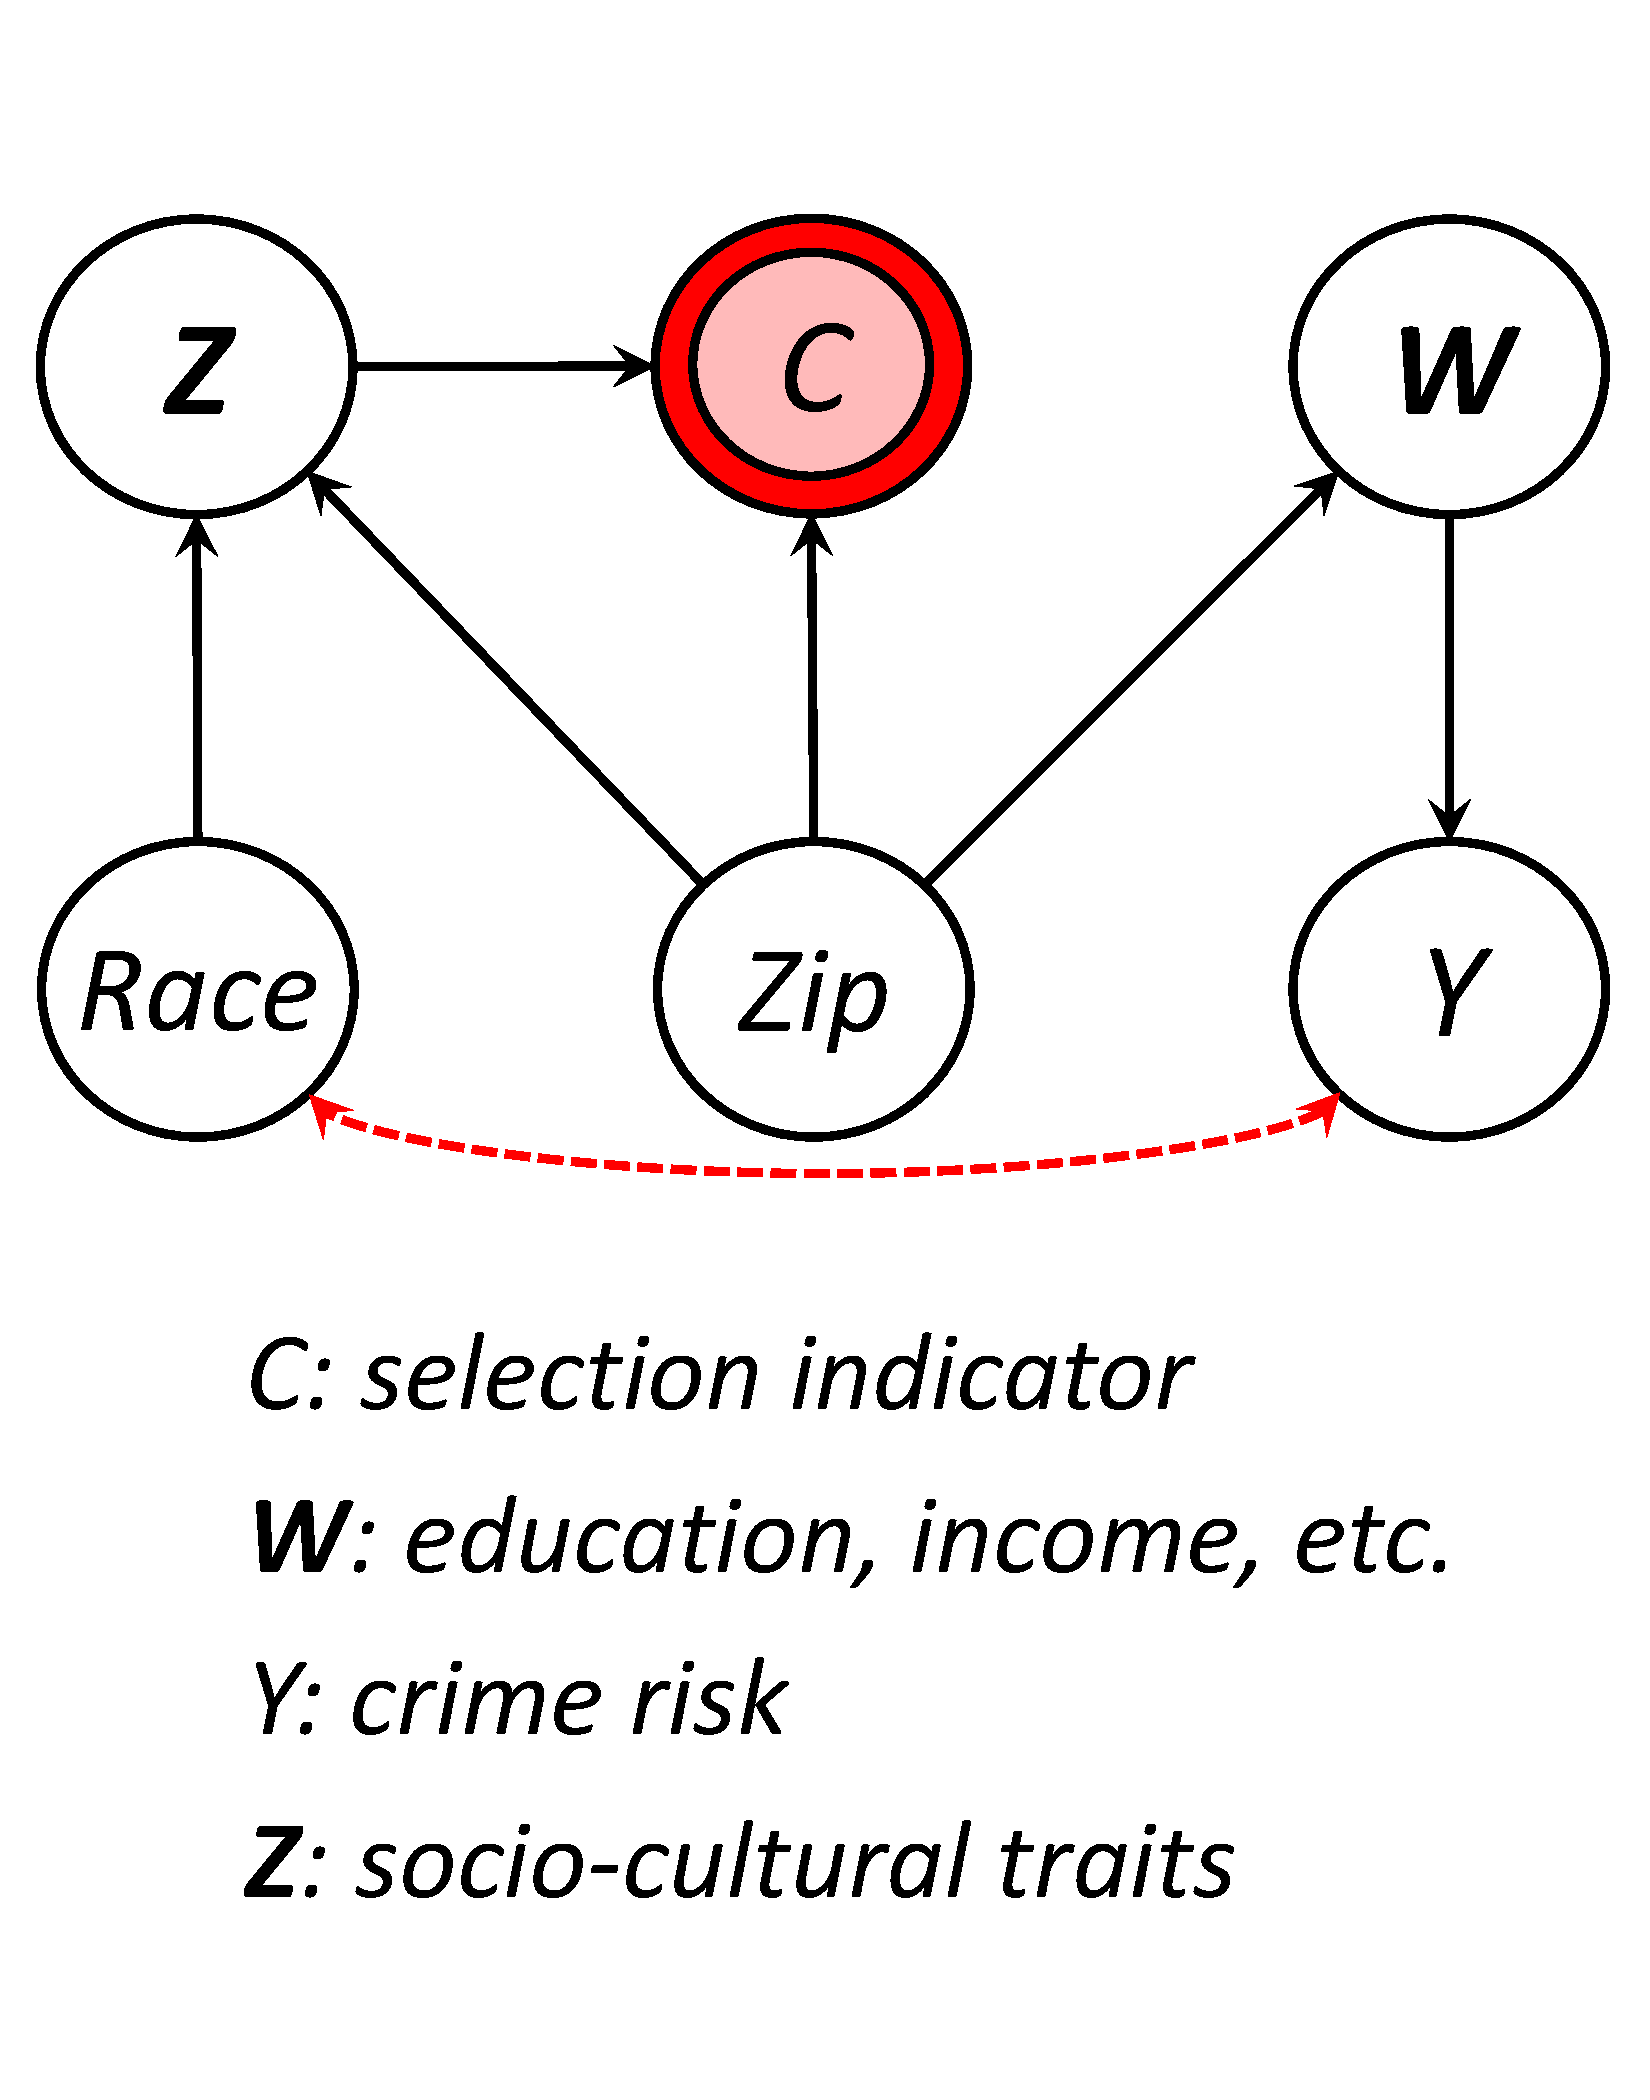
\includegraphics[width=\linewidth]{submissions/submission5/figs/selection-bias.pdf}
   \vspace{-.5cm}
   \caption{}
   \label{fig:selection-bias}
\end{subfigure}
\hfill
\begin{subfigure}[b]{0.24\textwidth}
   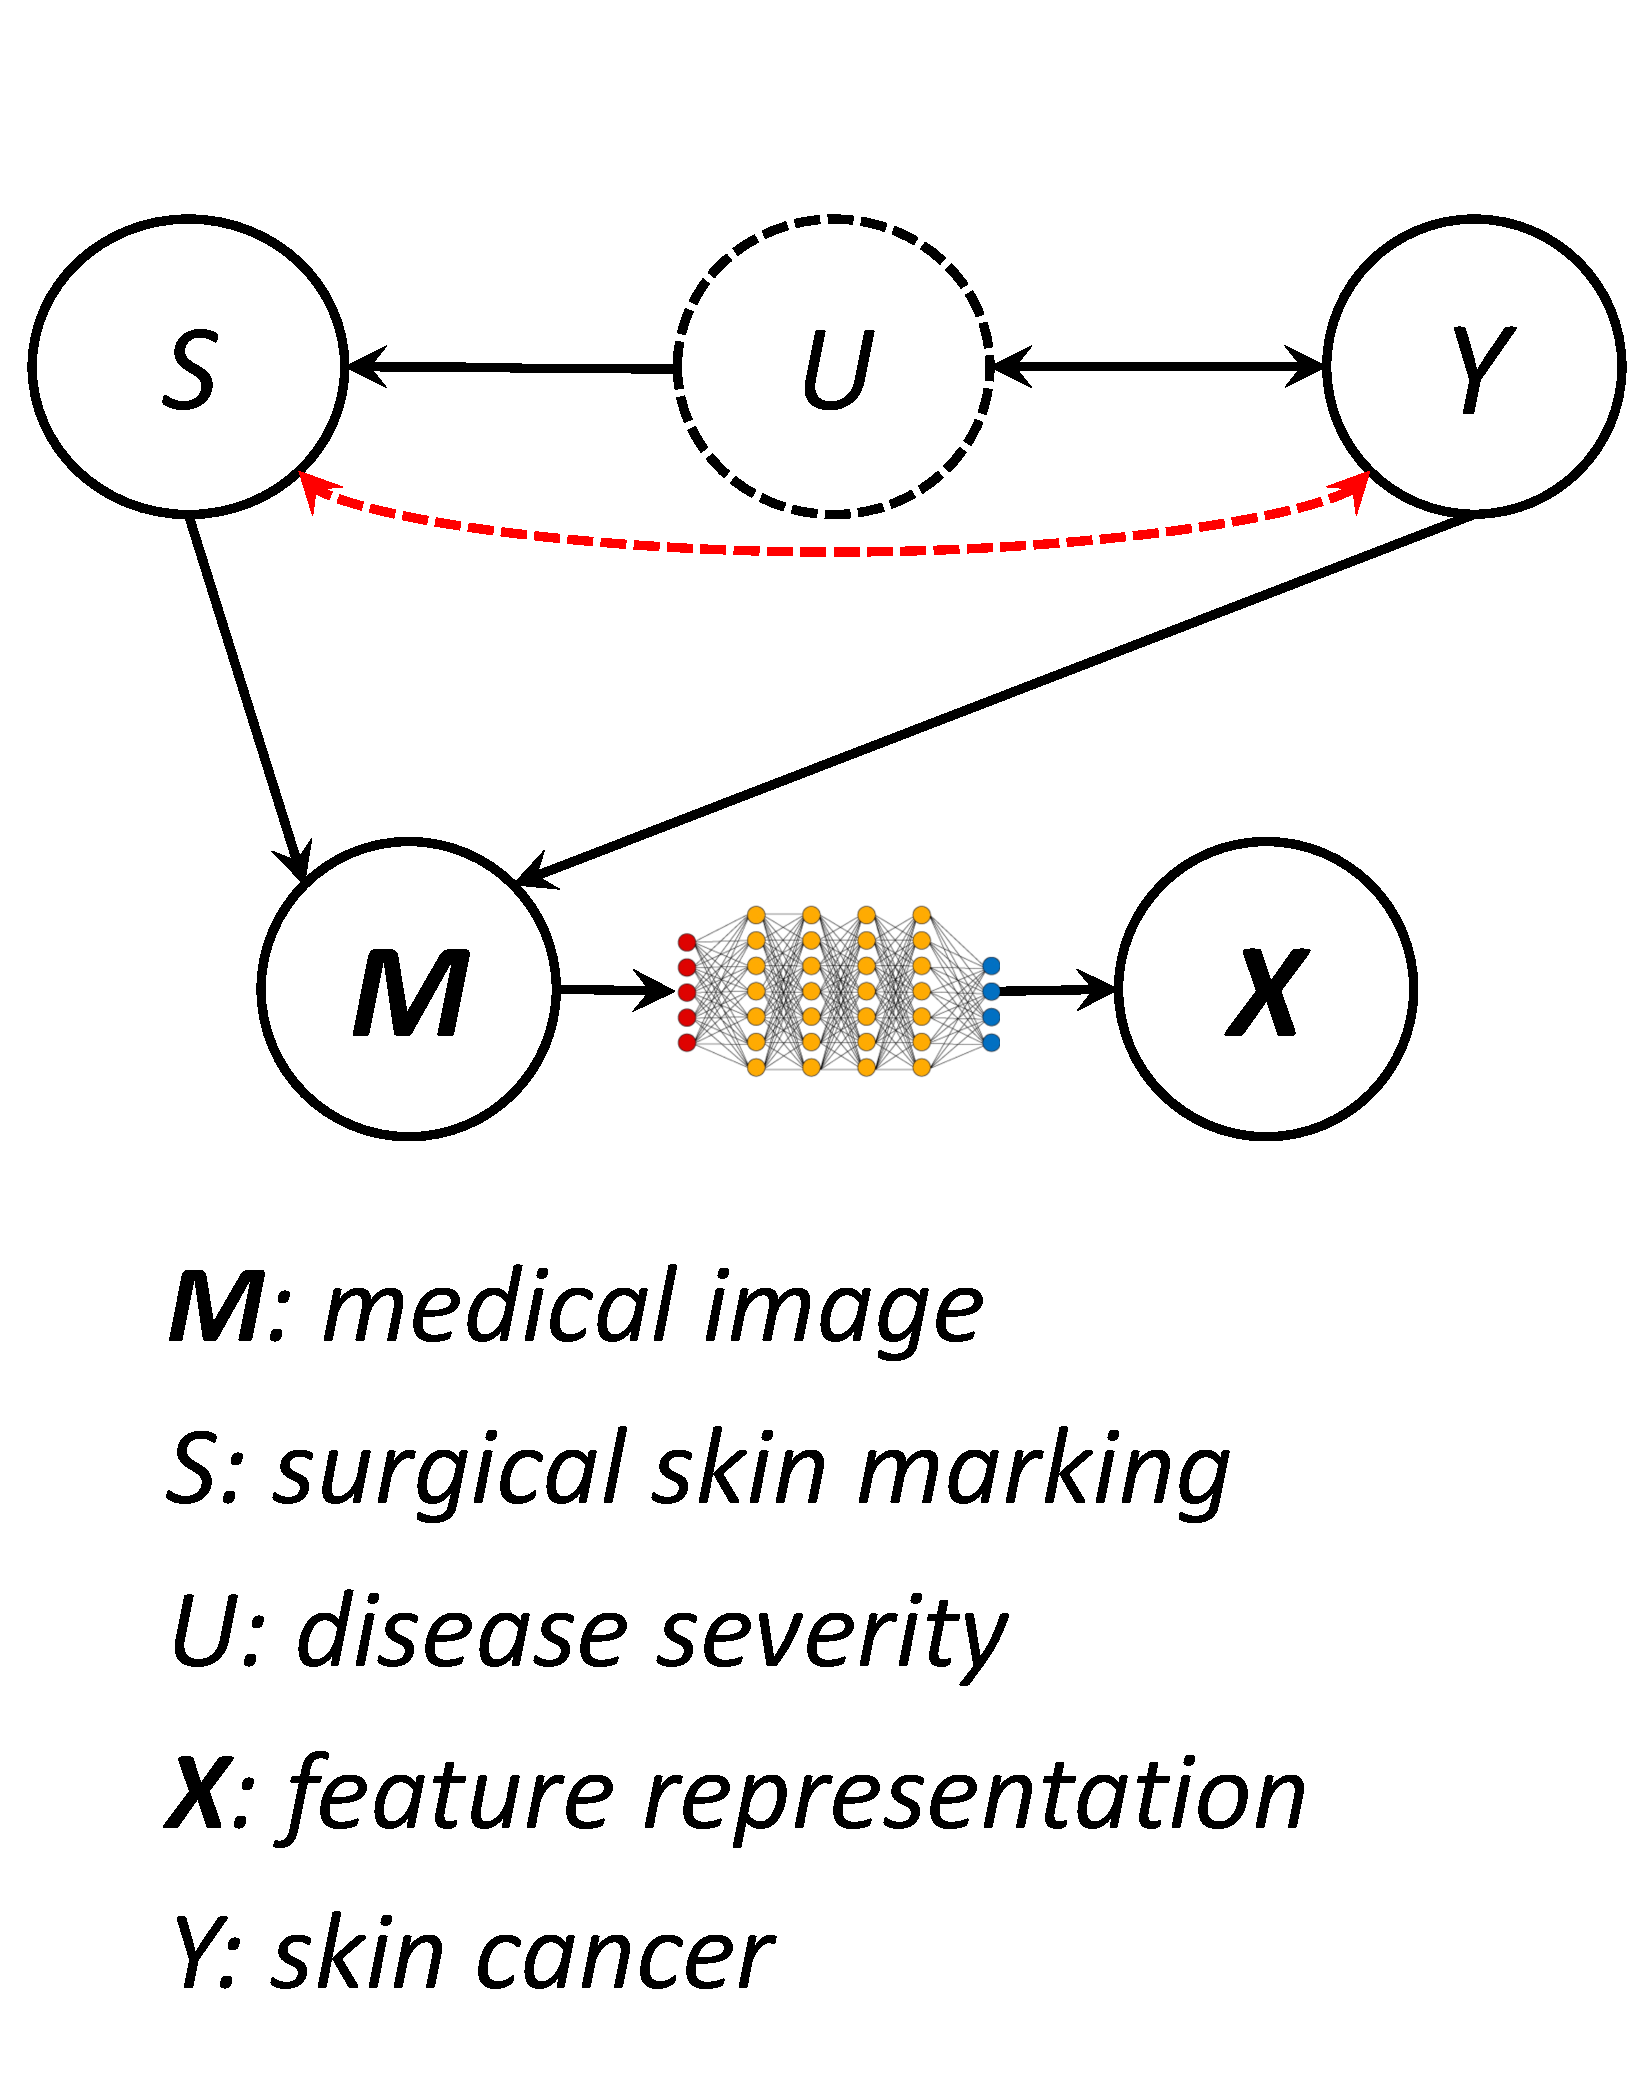
\includegraphics[width=\linewidth]{submissions/submission5/figs/confounding-bias.pdf}
   \vspace{-.5cm}
   \caption{}
   \label{fig:confounding-bias}
\end{subfigure}
\hfill
\begin{subfigure}[b]{0.24\textwidth}
   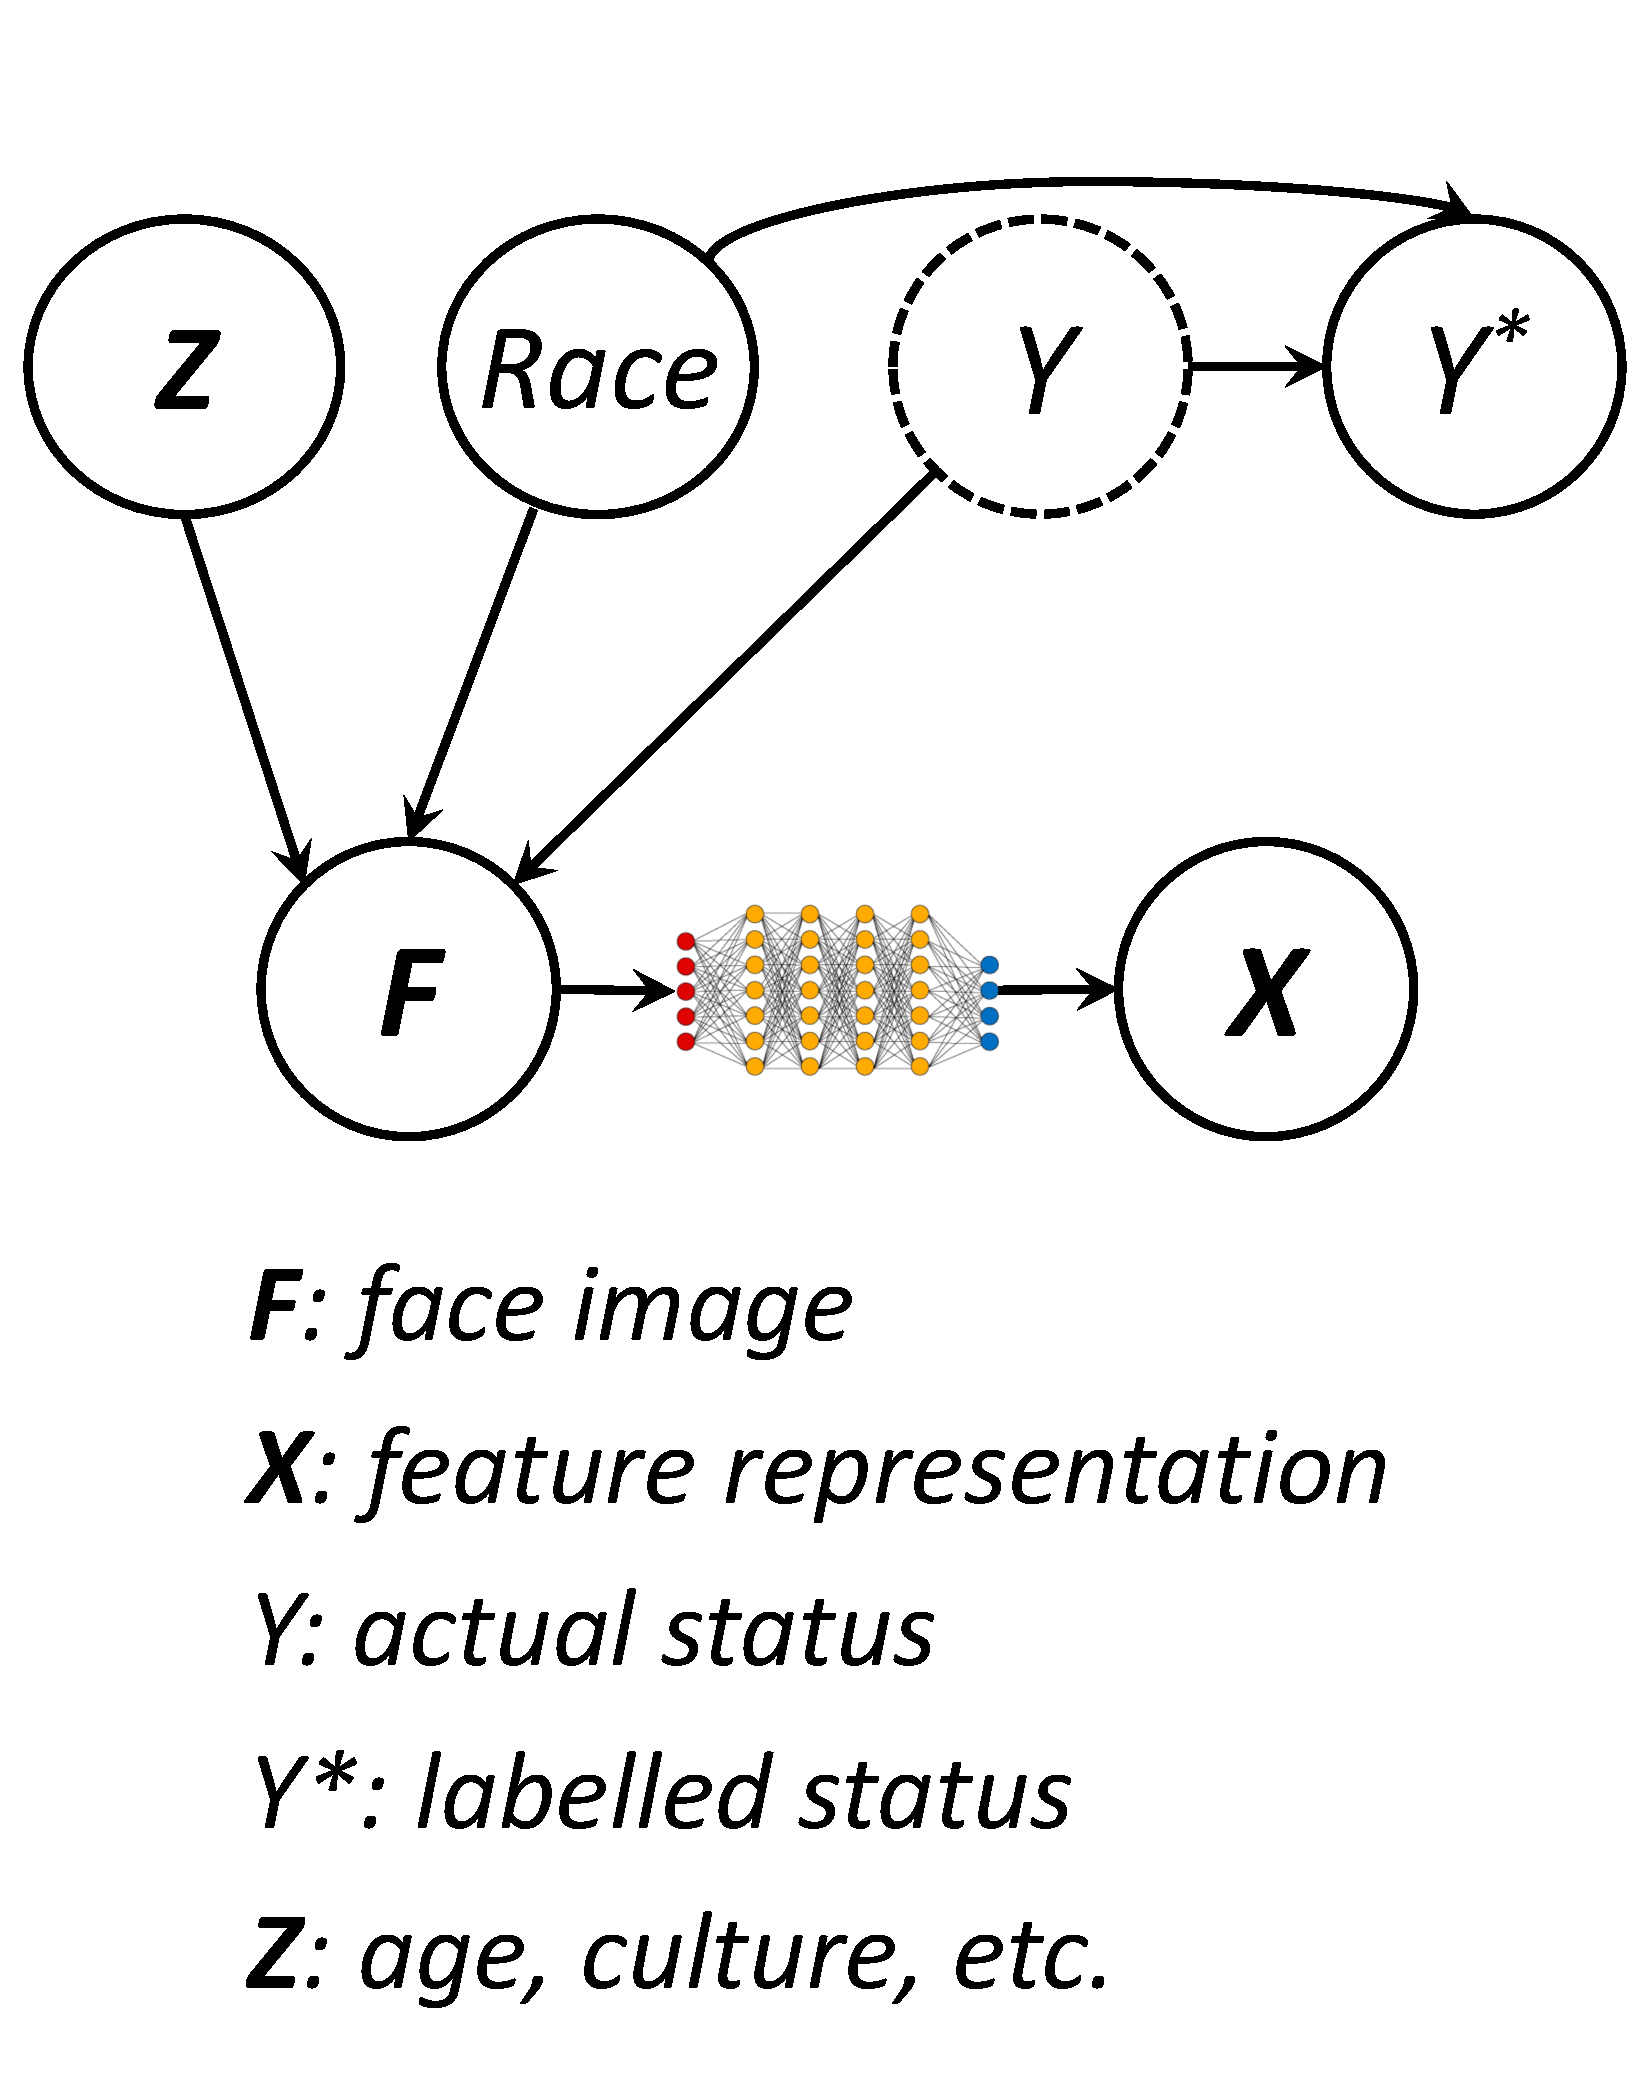
\includegraphics[width=\linewidth]{submissions/submission5/figs/label-measurement-bias.pdf}
   \vspace{-.5cm}
   \caption{}
   \label{fig:label-measurement-bias}
\end{subfigure}
\caption{(a) A causal diagram for modeling missing values in pediatric health studies. (b) A causal diagram for modeling selection bias in predictive policing. (c) A causal diagram for modeling confounding bias in medical imaging. (d) A causal diagram for modeling label bias in facial image labeling. The elements of a causal diagram are:
\protect\tikz{\protect\node[draw, line width=1pt, circle, fill=white , inner sep=2pt, minimum size=4mm] {};} representing observed attributes,
\protect\tikz{\protect\node[draw, line width=1pt, circle, fill=white , dotted, inner sep=2pt, minimum size=4mm] {};} denoting unobserved attributes,
\protect\tikz{\protect\draw[-latex, line width=1pt] (0,0) to[bend right] (1,0);} illustrating a causal dependency between two variables,
\protect\tikz{\protect\draw[<->, line width=1pt] (1.5,0) to[bend right] (2.5,0);} indicating a correlation due to common parent variables not included in the diagram, 
and \protect\tikz{\protect\draw[<->, red, dotted, line width=1pt] (3,0) to[bend right] (4,0);} signifying a spurious correlation due to data biases.}
\label{fig:data-biases-examples}
\end{figure}
\vspace{-.3cm}
\subsection{Modeling Bias due to Missing Data}
\subsubsection{Missing Values}

Missing values within a variable \(U\) can be efficiently represented using a binary missing indicator variable \(R_U\), which denotes the presence or absence of data in \(U\). Specifically, \(R_U = 1\) denotes a non-missing (present) value, whereas \(R_U = 0\) indicates a missing value. Furthermore, let \(U^*\) denote the observed dataset from \(U\), where missing entries are filled with a placeholder (e.g., null). We assume that only \(U\) is subject to missing values, with other variables' actual values being completely observed. The interaction between \(U\), \(R_U\), and \(U^*\) can be formally depicted as follows:

{\small
\[
U^* = \left\{
\begin{aligned}
&U, && \text{if } R_U = 1,\\
&\text{null}, && \text{if } R_U = 0.
\end{aligned}
\right.
\]
}

The subset of data that contains no missing values can be considered a sample from the distribution \(\Pr(\boldsymbol{V} \mid R_U = 1)\), where \(\boldsymbol{V}\) denotes the set of all variables. This implies that the subset of data without missing values is representative of the underlying distribution only if \(\Pr(\boldsymbol{V} \mid R_U = 1) = \Pr(\boldsymbol{V})\). The condition for this equality is that the occurrence of missing values is completely random, denoted as \((R_U \indep \boldsymbol{V})\), which suggests that \( R_U \) is causally independent of all other variables. However, in cases where missingness is not random, \( R_U \) is causally influenced by other variables. Such influence can be depicted in a causal graph with edges from influencing variables to \( R_U \), thus capturing the missingness pattern. Causal modeling, therefore, provides a comprehensive framework to explicitly identify the sources of non-random missing values and to understand their effects on the data distribution. It also aids in studying the sufficient and necessary conditions for the recoverability of missing data, thereby enhancing the robustness and applicability of data analysis in various contexts.

Next, we use a concrete example in credit risk assessment to show how non-random missing values can be modeled using causal diagrams and how this would affect the downstream ML model. 
\vspace{-.1cm}
\begin{example}[Credit Risk Assessment]\label{ex:causal-missing-val-children-health}  
   The causal diagram in Figure~\ref{fig:missing-value} depicts the scenario of missing values in loan application data, as discussed in Example~\ref{ex:missing-val-children-health}. This graph indicates that the actual loan repayment label \( Y \) is independent of demographic factors \( \boldsymbol{S} \), i.e., (\( \boldsymbol{S} \indep Y \)), suggesting that demographic information (\( \boldsymbol{S} \)) does not correlate with loan repayment (\( Y \)) in the underlying distribution (\( \Pr(Y \mid \boldsymbol{S}) = \Pr(Y) \)). The observed version of \( Y \), denoted as \( Y^* \), exhibits missingness influenced by individual demographics, reflecting that records from certain demographic groups are more prone to incompleteness due to historical biases. This relationship is captured in the causal diagram by the missingness variable \( R_Y \), which is dependent on the demographic information \( \boldsymbol{S} \). 
   Given the high correlation between the occurrence of missing values and demographics, any imputation method with errors could lead to a biased dataset. Consequently, the imputed labels \( Y^*_{\text{imp}} \) could become strongly correlated with demographic factors \( \boldsymbol{S} \). This outcome demonstrates the challenges in handling missing data, particularly when such missingness is non-randomly linked with demographic attributes. Consequently, models trained on this observed data are likely to be unfair, perpetuating historical biases.

\end{example}


Data imputation methods in practice often assume that missing data occurs either completely at random (MCAR) or at random (MAR), which suggests that the mechanism of missingness does not depend on the actual values of the variable that is missing~\cite{graham2012missing}. However, these methods may introduce bias when the missingness mechanism is not at random (MNAR), meaning the missingness of a variable is influenced by its own actual values or other latent variables. Such conditions render traditional imputation strategies prone to producing biased data as the original, true values of the data are typically not recoverable~\cite{guo2023sufficient,graham2012missing,pearl2013recoverability,lee2012recovery}. Consequently, ML models trained on this biased, imputed data inherit and perpetuate the bias, leading to unfair and unreliable outcomes. To mitigate these challenges, causal modeling has been instrumental in identifying both the necessary and sufficient conditions for effectively recovering from data missingness. Additionally, it aids in pinpointing which statistics or parts of the distribution can be recovered, or in determining the external information necessary for such recovery~\cite{mohan2021graphical}. The key to this approach lies in leveraging the invariance encoded by conditional independencies within the causal graph.


\vspace{-.3cm}
\paragraph{Fairness and Missing data:} 
Recent studies investigating the impact of imputation on algorithmic fairness under different missingness mechanisms reveal significant gaps. For instance, \cite{zhang2021assessing} presents theoretical results on fairness guarantees in the analysis of incomplete data, while \cite{jeanselme2022imputation} highlights common disparities in imputation quality across different demographic groups. 
Causal modeling has been pivotal in examining the relationship between fairness and the need to consider data missingness to achieve algorithmic fairness. In this vein, recent research has harnessed the power of causal modeling to unravel multivariate dependencies in datasets with missing data, exploring the sufficient and necessary conditions for recoverability of the distribution especially when multiple variables suffer from missing data~\cite{goel2021importance,nabi2022causal, mohan2021graphical}. In particular, \cite{goel2021importance} underscores that neglecting missing data can compromise the fairness of  ML  models, especially in high-stakes situations like loan decision-making. The authors of this study propose a novel algorithm with a decentralized decision-making process that only leverages recoverable conditional distributions when the joint data distribution is not recoverable. 


\vspace{-.3cm}
\subsubsection{Selection Bias}
The sampling or selection of tuples in a dataset can be modeled through a selection variable \( C \). This binary variable indicates whether a tuple is selected, i.e., the observed data can be viewed as a random sample from the distribution \( \Pr(\boldsymbol{V} \mid C=1) \), where \( \boldsymbol{V} \) represents the set of all variables. 
In the case of a completely random selection mechanism, where \( C \) is independent of \( \boldsymbol{V} \) (i.e., \( C \indep \boldsymbol{V} \)), the sampled data distribution \( \Pr(\boldsymbol{V} \mid C=1) \) is representative of the underlying distribution \( \Pr(\boldsymbol{V}) \). However, in the presence of selection bias, where the selection process is non-random, the selection variable \( C \) becomes dependent on other variables (i.e., \( C \nindep \boldsymbol{V} \)). This dependency is depicted in the causal graph by edges from variables that affect the selection of data to the variable 
\( C \), capturing factors influencing data selection. 
As a result, the sampled data becomes biased and not representative of the underlying distribution, as indicated by \( \Pr(\boldsymbol{V}) \neq \Pr(\boldsymbol{V} \mid C=1) \).



\vspace{-.3cm}
\begin{example}[Predictive Policing]\label{ex:selection-bias-police} 
Figure~\ref{fig:selection-bias} presents a simplified causal graph that captures the data collection process in predictive policing, where ML models are applied to predict crime. The graph encodes that crime risk \( Y \) is influenced by causal factors \( \boldsymbol{W} \) such as education and income, but is independent of Race. However, the graph also highlights the bias in police data, which often reflects biases from individuals' interactions with the police, influenced by socio-cultural traits and patrol frequency in their neighborhoods~\cite{brayne2015predictive,lum2016predict}. This reflects a case of non-random data selection, where the selection variable \( C \) is influenced by both the neighborhood (\( Zip \)) and socio-cultural traits (\( \boldsymbol{Z} \)), as depicted in Figure~\ref{fig:selection-bias}.
As a result, the police data can be viewed as a sample from \( \Pr(\boldsymbol{V} \mid C=1) \), where \( \boldsymbol{V} = \{Race, \boldsymbol{Z}, Zip, \boldsymbol{X}, Y\} \) represents the set of all variables. Due to selection bias, conditioning on \( C \) introduces a spurious correlation between race and crime (\( Race \nindep Y \mid C=1 \)) in the training data, a phenomenon known as collider bias, which is depicted by bidirectional dotted red arrows between them in the graph. Training an ML model on this biased dataset to predict crime risk is likely to learn and propagate this spurious correlation, utilizing race in predicting crime, leading to unfair and inaccurate outcomes.
\end{example}


Significant efforts in  ML  have been directed towards mitigating selection bias, employing various techniques including causal modeling to establish when it is fundamentally possible to recover from such biases~\cite{bareinboim2012controlling, bareinboim2014recovering}.  Within this scope, a prominent manifestation of selection bias is termed covariate shift, which occurs when there is a discrepancy in the distribution of features $\boldsymbol{X}$ between the training and test data, while the conditional distribution $\Pr(Y \mid \boldsymbol{X})$ remains constant.
This phenomenon often arises when training data suffers from selection bias where the selection mechanism is independent of the label $Y$. 
This implies that the selection variable does not directly depend on the training label $Y$ and is d-separated from it by $\boldsymbol{X}$ in the causal diagram.


\vspace{-.3cm}
\paragraph{Fairness and Selection bias:}
Recent work in  ML  has focused on the interaction between algorithmic fairness and selection bias~\cite{liu2014robust,huang2006correcting,cortes2008sample,rezaei2020robust,du2021robust}. These works, including inverse propensity scoring and density ratio estimation, often rely on specific assumptions about the underlying data distribution or the need for access to unbiased samples, a requirement that can be restrictive in practical scenarios. This challenge is particularly pronounced in sensitive areas such as predictive policing, healthcare, and finance, where inherent biases in these fields make obtaining unbiased data samples impossible. However, it is often more practical to acquire background knowledge about the data collection process in these domains. Such knowledge can be effectively represented through causal diagrams. In this vein, \cite{singh2021fairness} introduces a method that uses causal diagrams to mitigate model unfairness, especially under covariate shift scenarios, although this method is applicable primarily to addressable graphs that satisfy certain graphical conditions.


To overcome the limitations encountered in previous methods, a recent study \crab~\cite{zhu2023consistent} introduces an approach for constructing fair ML models in the presence of selection bias, without the need for an unbiased dataset. Instead of relying on stringent assumptions or unbiased samples from the underlying distribution, \crab only requires partial knowledge about the data collection process. This approach makes it more practical compared to other methodologies that necessitate more restrictive conditions. Next, we will review \crab as a case study to illustrate how causal reasoning can be effectively utilized to develop ML models that maintain fairness in the underlying distribution, even when faced with selection bias.

\begin{figure}[t]
    \centering
    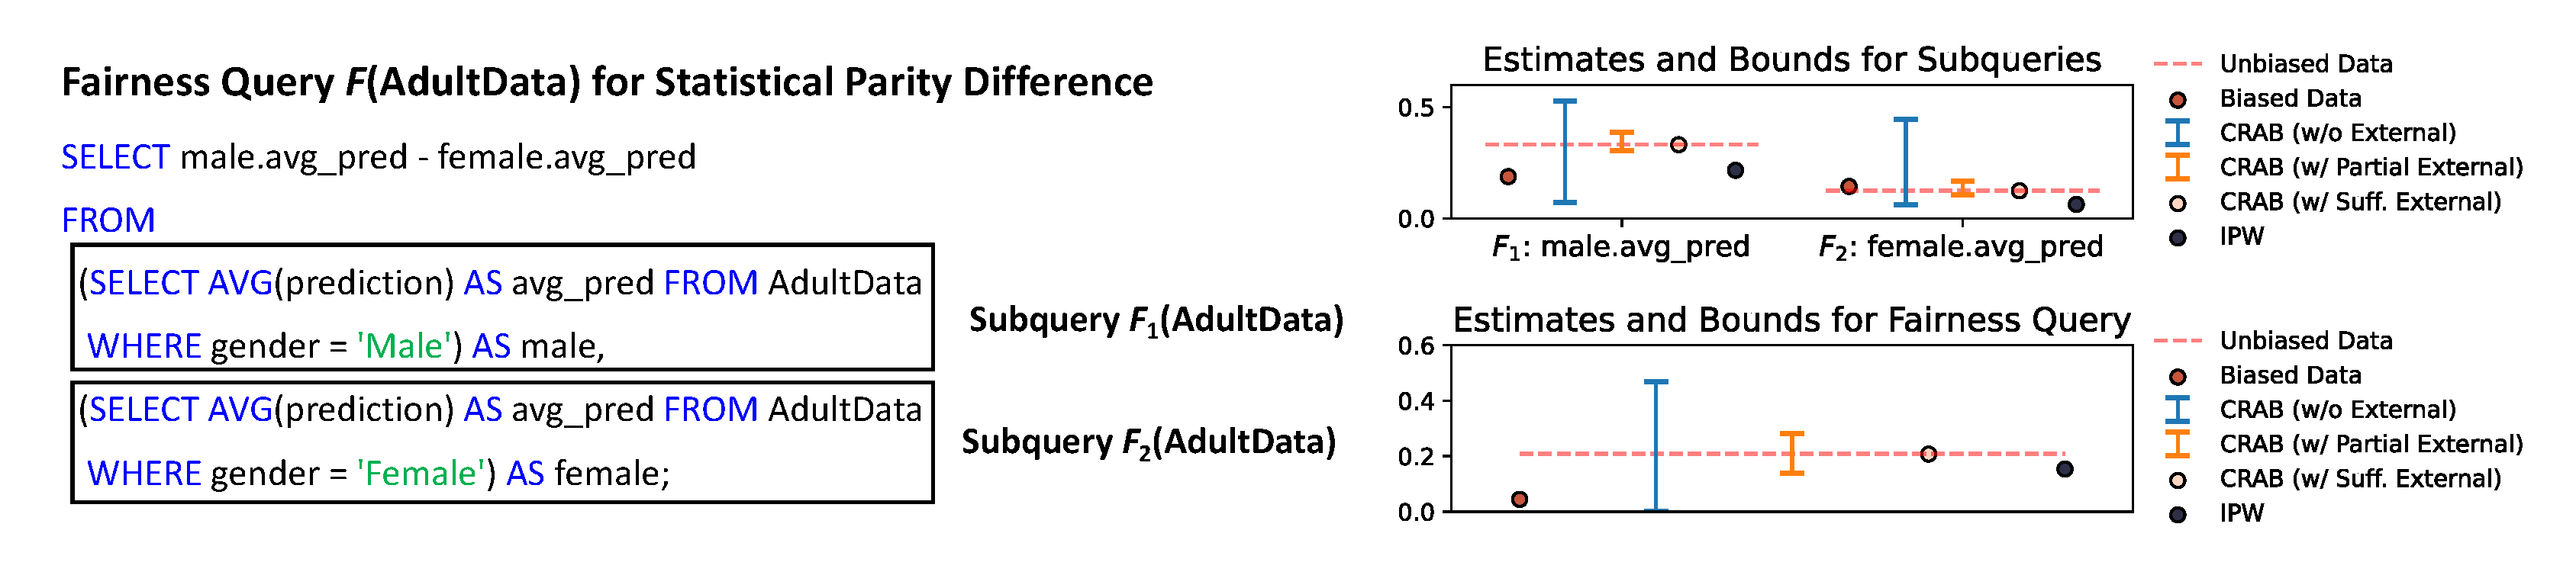
\includegraphics[width=\linewidth]{submissions/submission5/figs/bound_comp.pdf}
    \vspace{-8mm}
    \caption{
    Comparative analysis of the consistent ranges obtained through CRA, alongside various estimates and the ground truth for the fairness query in the presence of selection bias in training data. In these plots, the red lines denote the fairness queries calculated using unbiased data. The fairness queries computed using biased data serve as a biased estimate of the unbiased fairness query. Another estimate of unbiased fairness query uses inverse propensity scores to re-weigh the data when evaluating fairness queries (\ipw)~\cite{cortes2008sample}. The consistent ranges derived by \crab with varying availability of external data are shown. Specifically, given sufficient external data, the consistent upper and lower bounds overlap~\cite{zhu2023consistent}.}
    \label{fig:boundcomp}
\end{figure}

\vspace{-.3cm}
\subsubsection{Consistent Range Approximation for Building Fair Models under Selection Bias}
\texttt{CRAB} presents a framework for developing fair models under selection bias, tailored to enforce fairness definitions that can be captured by conditional independence constraints, such as conditional statistical parity, equality of odds, and predictive parity~\cite{zafar2017fairness}. Central to this framework is \emph{fairness queries}, which assess the fairness of a classifier $h$, which will be reviewed next.
\vspace{-.3cm}
\paragraph{Fairness query:}
Let $\classifier$ be a binary classifier with a protected attribute $\ProtectedAttr \in \boldsymbol{X}$, the \emph{fairness query} is a measure used to assess the fairness violation of a model $h$ wrt. the conditional statistical parity. It is defined based on a set of admissible attributes $\Admis$ and a population $\Omega$ with support $\boldsymbol{X} \times Y$:

{\small$$
\begin{aligned}\label{eq:fairnessquery}
\sCondDemoParityDist{\dist}
= \frac{1}{ 2 \ \lvert\Admis\rvert}  \sum_{ \substack{y\in\Dom{Y},\\ \admis\in\Dom{\Admis}} }\big\lvert\pr_{\dist }(h(\boldsymbol{x})=y\mid \privG, \admis)-\pr_{\dist}(h(\boldsymbol{x})=y\mid\protG, \admis)\big\rvert.
\end{aligned}
$$}

It can be easily verified that for a model $h$ to satisfy conditional statistical parity in a target population $\dist$, it must fulfill the condition $\sCondDemoParityDist{\dist} = 0$. In this context, a fairness query is essentially the average dependency between the model's output and sensitive attributes, once adjustments have been made for admissible attributes. In practice, given a data $D_\dist$ sampled from the distribution $\dist$, the fairness query $\sCondDemoParityDist{\dist}$ can be computed through the empirical fairness query $\seCondDemoParityDist{D_\dist}$, which can be seen as an empirical estimate of $\sCondDemoParityDist{\dist}$. Specifically, in the context of binary classification, $\seCondDemoParityDist{D_\dist}$ can be calculated by:
{\small$$
\begin{aligned}\label{eq:empiricalfairnessquery}
\seCondDemoParityDist{D_\dist}= \frac{1}{\ \lvert\Admis\rvert} \sum_{\admis\in\Dom{\Admis}} \Bigg\lvert \frac{\sum_{\boldsymbol{x}\in\NPos{\privG, \admis}}{\classifier(\boldsymbol{x})} }{\lvert\NPos{\privG, \admis}\rvert}-
\frac{\sum_{\boldsymbol{x}\in\NPos{\protG, \admis}}{\classifier(\boldsymbol{x})} }{\lvert\NPos{\protG, \admis}\rvert}\Bigg\rvert
\end{aligned}
$$}
where $\NPos{s, \admis}$ denotes the set of data points in $D_\dist$ with positive labels, protected attribute values $\ProtectedAttr=\protectedAttr$ and admissible attributes value $\Admis=\admis$. {For example, Figure~\ref{fig:boundcomp} presents an empirical fairness query that measures the model's violation of statistical parity on the adult data.} In order to avoid sampling variability, in the subsequent, we assume samples are sufficiently large such that $\seCondDemoParityDist{D_\dist}\approx\sCondDemoParityDist{\dist}$ and use them interchangeably.

{Building models that are fair on the target population $\Omega$ requires to achieve $\sCondDemoParityDist{\Omega}=0$. However, in practice, we only have access to the biased data $D_\Delta$ sampled from the population $\Delta$ that suffers from selection bias. 
Using this biased data $D_\Delta$ to evaluate fairness query gives $\seCondDemoParityDist{D_\Delta}$, which is a biased and inaccurate estimate of the actual unfairness $\sCondDemoParityDist{\Omega}$. 
Furthermore, mitigating unfairness based on this biased estimate will result in a model that is fair on the biased training data ($\sCondDemoParityDist{\Delta}=0$), while being unfair when deployed to the unbiased target population ($\sCondDemoParityDist{\Omega}\neq0$).
Nevertheless, without external data about the unbiased target population $\Omega$, it's almost impossible to accurately estimate $\sCondDemoParityDist{\Omega}$. 

In addressing the challenge of answering fairness queries from data affected by selection bias, the situation is akin to query answering on incomplete datasets, where complete and accurate responses are unattainable due to missing information. This challenge is tackled using an approach inspired by the concepts of possible worlds and consistent query answering~\cite{console2020coping,fan2012foundations,feng2021efficient,koutris2018consistent}. \texttt{CRAB} utilizes this methodology by considering every conceivable underlying population or ``possible world" from which the training data could have been obtained. Conceptually, \texttt{CRAB} computes the fairness query in each possible world and then uses these computations to establish a range for the fairness query by determining upper and lower bounds for unbiased fairness query answers. To generate tight and meaningful ranges, \texttt{CRAB} incorporates auxiliary information, which helps in narrowing down the range of potential underlying distributions. This approach is crucial for accurately evaluating fairness in models where the data is compromised by selection bias, ensuring a more reliable and valid assessment of fairness.


\vspace{-.3cm}
\paragraph{Auxiliary information and possible repairs:}
The auxiliary information that \crab incorporates includes the {\em causal diagram} that represents the collection process of the biased data, and a set of {\em external data sources} that can potentially provide {\em partial} information about the underlying distribution $\underlyingDist$.
Intuitively, the causal diagram encodes the causes of selection bias, i.e., which variables affect the tuple selection, while the external data source can be used to compute unbiased statistics about the underlying distribution.
\crab captures the space of possible unbiased, complete data using the notion of {\em possible repairs}.
Formally, given a biased dataset $\bdata$, the set of possible repairs of $\bdata$, denoted as $\repairs(\bdata)$, is defined as the set of all datasets $D$ with the same schema as $\bdata$ such that: (1) $D \supsetneq \bdata$ and (2) $D$ is consistent with $\bcdag$ and $\auxdata$, i.e., it satisfies the constraints posed by the auxiliary information.
Specifically, all repairs in $\repairs(\bdata)$ must adhere to the conditional independences encoded in the causal diagram, and the unbiased statistics derived from $\auxdata$.
Note that \crab does not compute each of the possible repairs. Instead, the concept of possible repairs is used as a framework for addressing the incompleteness of information in the presence of selection bias. The problem of consistent range approximation is built upon the concept of possible repairs.
}


\vspace{-.3cm}
\paragraph{Consistent range approximation:}
The consistent range approximation (CRA) computes the consistent upper bound (CUB) and consistent lower bound (CLB) of the fairness query $\sCondDemoParityDist{\Omega}$.
Similar to consistent query answering in databases~\cite{bertossi2006consistent,dixit2021consistent}, CRA considers the space of all possible repairs, which stands for possible ways to complete the biased data $D_\Delta$. Specifically, 
\vspace{-.15cm}
{\small
\begin{align*}
    \lowerbound = \min_{D\in \repairs(\bdata)} \hat{\digamma} (D), ~~~~\upperbound=\max_{D\in \repairs(\bdata)} \hat{\digamma} (D)
\end{align*}
}
\vspace{-.35cm}


As mentioned, CRA does not compute each of the possible repairs, but utilizes the conditional independence conditions encoded in the causal diagram, which every possible repair must satisfy, to derive closed-form solutions for the range of fairness query answers. 
This ensures that the actual unfairness of the model on the underlying distribution will fall within this computed range, i.e. $\sCondDemoParityDist{\dist}\in [\lowerbound,\upperbound]$. This range is referred to as the \emph{consistent range}.
Furthermore, CRA can integrate varying levels of external data sources about the underlying distribution, enabling the derivation of more precise consistent ranges. This property makes \crab a practical solution for addressing selection bias.

It is worth noting that the external data source is not mandatory for CRA. In the absence of external data sources, \cite{zhu2023consistent} provides the closed-form CUB and CLB leveraging merely the conditional independence condition encoded in the causal diagram. We use the example of police data to demonstrate CRA in the absence of external data sources. For simplicity, we illustrate the CRA of fairness query wrt. statistical parity, where $\Admis=\emptyset$.
\begin{example}[CRA on the Predictive Policing Data]\label{ex:cra-police}
Continuing with Example~\ref{ex:selection-bias-police}, assume the protected attribute $Race\in\{white,non\text{-}white\}$ and the label, crime risk $Y\in\{low\ risk,high\ risk\}$. 
In this case, the fairness query wrt. statistical parity notion can computed by:

\vspace{-.2cm}
{\small\begin{equation}\label{eq:spd}
\sCondDemoParityDist{\Omega}=\pr_{\dist }(low\ risk\mid white)-\pr_{\dist}(low\ risk\mid non\text{-}white).
\end{equation}}
\vspace{-.3cm}

The CUB of $\sCondDemoParityDist{\Omega}$ can be derived by combining the upper bound of $\pr_{\dist }(low\ risk\mid white)$ and the lower bound of $\pr_{\dist}(low\ risk\mid non\text{-}white)$. First, we show how $\pr_{\dist }(low\ risk\mid white)$ is upper bounded.
As presented in Figure~\ref{fig:selection-bias}, the selection variable $C$ is influenced by $ZIP$ and $\textbf{Z}$. Let $\boldsymbol{U}=\Pa(C)=\{\boldsymbol{Z},ZIP\}$, we have the conditional independence condition encoded in the causal diagram: $\mbox{$(C\indep \boldsymbol{V}\mid \boldsymbol{U})$}$, where $\boldsymbol{V}$ is the set of all variables.
The following holds due to this conditional independence:
{\small\begin{equation}\label{eq:ci}
    \pr_{\underlyingDist}(low\ risk \mid white,\boldsymbol{u})=\pr_{\underlyingDist}(low\ risk \mid white,\boldsymbol{u},C=1)=\pr_{\Delta}(low\ risk \mid white,\boldsymbol{u}).
\end{equation}}
The upper bound of $\pr_{\dist }(low\ risk\mid white)$ can be derived by applying the law of total probability and Eq.~\ref{eq:ci}:

\vspace{-.3cm}
{\small\begin{flalign}\label{eq:upperbound}
    \indent&\begin{aligned}
        \pr_{\dist }(low\ risk\mid white)
        &= \sum_{\boldsymbol{u} \in \Dom{\boldsymbol{U}}} \pr_{\underlyingDist}(low\ risk \mid white,\boldsymbol{u})\pr_{\underlyingDist}(\boldsymbol{u}\mid white)\\
        & = \sum_{\boldsymbol{u} \in \Dom{\boldsymbol{U}}} \pr_{\popul}(low\ risk \mid white,\boldsymbol{u})\pr_{\underlyingDist}(\boldsymbol{u}\mid white)\\
        &\leq \sum_{\boldsymbol{u} \in \Dom{\boldsymbol{U}}} (\max_{\boldsymbol{u^*} \in \Dom{\boldsymbol{U}}}\pr_{\popul}(low\ risk \mid white,\boldsymbol{u^*}))\ \ \pr_{\underlyingDist}(\boldsymbol{u}\mid white)\\
        &= \max_{\boldsymbol{u^*} \in \Dom{\boldsymbol{U}}}\pr_{\popul}(low\ risk \mid white,\boldsymbol{u^*})\sum_{\boldsymbol{u} \in \Dom{\boldsymbol{U}}}\pr_{\underlyingDist}(\boldsymbol{u}\mid white)\\
        &= \max_{\boldsymbol{u^*} \in \Dom{\boldsymbol{U}}}\pr_{\popul}(low\ risk \mid white,\boldsymbol{u^*}).
    \end{aligned}&&
\end{flalign}}
\vspace{-.3cm}

Similarly, one can derive a lower bound for \(\pr_{\dist}(\text{low risk} \mid \text{non-white})\), resulting in the subsequent formulation for the CUB of the fairness query:

{\small$$\sCondDemoParity\leq \upperbound=\max_{\boldsymbol{u^*} \in \Dom{\boldsymbol{U}}}\pr_{\popul}(low\ risk \mid white,\boldsymbol{u^*})-\min_{\boldsymbol{u^*} \in \Dom{\boldsymbol{U}}}\pr_{\popul}(low\ risk \mid non\text{-}white,\boldsymbol{u^*}).$$}

Furthermore, if sufficient external data sources which enable computing the unbiased statistics $\pr_{\dist}(\boldsymbol{u}\mid white)$ are available, CRA is able to directly estimate $\sCondDemoParityDist{\dist}$.

\end{example}

The above results demonstrate how CRA gives consistent ranges with no or sufficient external data. 
In practice, one may have access to a level of external data that falls in between these two extremes. For instance, we might not have access to the external data about socio-cultrual traits $\boldsymbol{Z}$, thus only being able to compute the unbiased probabilities $\pr_{\Omega}(ZIP\mid Race)$. \crab also provides closed-form consistent ranges when having partial access to external data, including this case.
Next, we empirically compare the various estimates of the fairness query with the CLBs and CUBs obtained through CRA on real-world data. We focus on the CLBs and CUBs computed when having no or sufficient external data, as they have been introduced in Example~\ref{ex:cra-police}. 
\vspace{-0.2cm}
\begin{example}
    {Figure~\ref{fig:boundcomp} presents the comparison between consistent ranges and the estimates of the model's unfairness on the unbiased distribution. The adult data~\cite{adult}, which contains financial and demographic data to predict if an individual’s income exceeds $50K$, is used for model training and testing. Specifically, the training data is injected with selection bias, where the selection depends on gender, age, and relationship. 
    In the example, the consistent range of the fairness query can be computed based on the consistent ranges of its sub-queries. When unbiased external data is unavailable, the fairness query computed using biased data shows significant inaccuracy, especially for subquery $\digamma_2$.
    Nevertheless, in the absence of unbiased external data, \crab guarantees to upper and lower bound the actual query answer on the underlying distribution.
    When the unbiased external data is leveraged, \ipw still deviates from the unbiased fairness query. In contrast, given sufficient external data (a subset of unlabeled data used by \ipw), the consistent upper and lower bounds derived by \crab overlaps, resulting in an accurate estimate of the unbiased fairness query. 
    In addition, the consistent ranges obtained with partial external data demonstrate the effectiveness of incorporating limited unbiased external data for deriving tighter consistent ranges.
    The results imply that (1) the consistent ranges always guarantee to bound the actual unfairness of the ML model, and (2) given external data about unbiased distribution, \crab is able to derive tighter bounds or estimates of the unbiased fairness query.}
\end{example}

The CUBs of fairness queries can be seen as the models' worst-case unfairness given available information about the underlying distribution. Therefore, CUBs can be used to train certifiably fair ML models by incorporating them into the loss function. In addition to the \crab system, \cite{zhu2023consistent} also presents a theoretical analysis of the impact of selection bias on the fairness of ML models and establishes necessary and sufficient graphical conditions on the data collection causal diagram under which the selection bias leads to unfair ML models.


\subsection{Confounding Bias}
Confounding bias presents challenges in ML when a latent variable \(C\) confounds some observed features \(S\) with the training label \(Y\), distorting their association. For example, in healthcare data, suppose \(S\) represents lifestyle factors or genetic predispositions, \(Y\) is the disease training label, and \(C\) encompasses unrecorded environmental factors like exposure to pollutants or access to healthcare facilities. Reliance on \(S\) for predicting \(Y\) can render ML models unreliable due to unstable correlations across different settings~\cite{zhang2021deep}. Furthermore, when \(S\) includes sensitive attributes, confounding bias can introduce biases that unfairly impact certain groups, especially if \(C\) relates to socioeconomic factors such as income level or education, thereby exacerbating disparities.

\vspace{-0.3cm}
\begin{example}[Medical Imaging]\label{ex:causal-confounding}
Continuing with the application of skin cancer detection in Example~\ref{ex:confounding}. The causal modeling of confounding bias is shown in Figure~\ref{fig:confounding-bias}.
In the causal diagram, the presence of a surgical skin marking ($S$) does not causally contribute to skin cancer ($Y$) as there are no edges between them. However, they become correlated in the data due to the confounding of disease severity ($U$). 

Since ML models learn correlation instead of causation, this non-causal spurious correlation between the presence of surgical skin markings and skin cancer will be learned and lead to inaccurate predictions. In particular, the model will have a high false positive rate on patients with other severe diseases, who are also likely to have surgical skin markings.
\end{example}

\vspace{-0.8cm}
\paragraph{Fairness, Robustness, and Confounding Bias:} Confounding bias poses a significant challenge across the board, particularly impacting the robustness and fairness of algorithmic models. The crux of efforts in algorithmic fairness is to ensure that sensitive attributes and training labels remain independent, conditioned on a subset of observed features, thus aiming to nullify spurious correlations brought about by unobserved confounding biases~\cite{salimi2019capuchin,galhotra2022causal,ma2023learning}. Achieving such independence (\(S \indep Y \mid X\)), as exemplified in Example~\ref{ex:causal-confounding}, is vital for preventing reliance on non-causal features like surgical markings for predictions, which enhances both the fairness and robustness of models. A variety of approaches have been developed to enforce conditional independence, ranging from feature selection methods that mitigate spurious correlations~\cite{galhotra2022causal}, counterfactual data augmentation techniques that elucidate causal relationships and generate varied counterfactual scenarios~\cite{ma2023learning}, to minimal repair strategies such as \textit{Capuchin} for data adjustment in compliance with Multivalued Dependency (MVD)~\cite{salimi2019capuchin}. Furthermore, in-processing techniques play a crucial role, incorporating strategies such as integrating conditional mutual information into the loss function~\cite{seo2022information}, employing adversarial mechanisms for confounding-invariant feature extraction~\cite{zhao2020training}, and developing feature representations that achieve conditional independence~\cite{xu2020algorithmic}. Ultimately, causal inference stands as a foundational strategy for modeling confounding bias and securing the requisite conditional independence, thus bolstering the efforts to enhance fairness and ensure robustness against confounding bias and spurious correlations in algorithmic models.

\vspace{-0.4cm}
\subsection{Measurement Bias}
\vspace{-.15cm}

Given a variable $U$ affected by the measurement error, we can create a variable $U^*$ indicating the collected or observed values, while the actual variable $U$ is unobserved. 
When measurement errors are non-random, the values of the observed variable $U^*$ often depend on its actual value $U$ and other variables. 
The observed data suffering from this measurement bias can be seen as a random sample from $\Pr(\boldsymbol{V}\setminus \{U\}, U^*)$ where $\boldsymbol{V}$ denotes the set of all variables. It is only representative of the underlying distribution when $\Pr(\boldsymbol{V})=\Pr(\boldsymbol{V}\setminus \{U\}, U^*)$, which rarely holds in practice.
In the context of  ML, the label variable $Y$ often suffers from mismeasurement and appears to be biased, which degrades the performance of downstream ML models~\cite{jiang2020identifying}.
Next, we will discuss an example of label bias existing in the medical imaging data.
\vspace{-.15cm}
\begin{example}[Modeling Label Bias]\label{ex:label-bias}
    Continuing with the scenario of facial identification in Example~\ref{ex:label-bias}. Figure~\ref{fig:label-measurement-bias} presents the causal modeling of label bias in this application. Ideally, the actual label $Y$ and the sensitive attribute $Race$ are independent ($\mbox{$Y\indep Race$}$). 
    However, due to the inadvertent bias during the labeling, the observed label $Y^*$ is influenced by both $Race$ and $Y$, resulting in the correlation between race-related facial features and labels in the observed data ($\mbox{$Y^*\nindep Race$}$). Consequently, models trained on this biased observed data will predict based on race-related facial features, leading to inaccuracies and unfairness.
\end{example}

The general problem of measurement bias has been studied recently, particularly in the context of causal inference. Through structural equation modeling, \cite{King-Kallimanis2010Using} detects measurement bias in longitudinal health-related data. In contrast, \cite{Barendse2014Measurement} applies Bayesian factor analysis to effectively detect both uniform and non-uniform measurement bias, with high detection rates in cases where an observed violator is present. 
To eliminate the systematic bias induced by measurement errors, \cite{pearl2012measurement} highlights several algebraic and graphical methods that work under different assumptions about the error mechanism. 
Beyond the broader issue of measurement bias, a range of research specifically targets the challenge of unfairness stemming from label bias.

\vspace{-.5cm}
\paragraph{Fairness and Label Bias:} Addressing label bias in ML necessitates innovative optimization and modeling strategies. \cite{jiang2020identifying} tackles this by positing that the distribution of biased labels should closely match the true distribution in terms of KL divergence, subject to the observed level of unfairness. They approach this through a constrained optimization problem, adjusting data weights to mitigate label bias while aiming for minimal alteration. \cite{zhang2023iflipper} approaches fairness through a label-flipping optimization problem, designed to adjust labels for individual fairness with minimal changes, formulated as a mixed-integer quadratic programming problem. This is further refined to an integer linear programming challenge, with \cite{zhang2023iflipper} providing approximate yet theoretically grounded solutions. On another front, \cite{zhang2023mitigating} focuses on identifying label inaccuracies by associating low self-confidence in model predictions with potential errors, utilizing confidence intervals for selective data refinement.  These methods, while effective, often rely on simplifying assumptions, such as a minimal number of mislabeled instances, and do not fully confront measurement bias directly. However, advancements in causal modeling offer a principled approach to constructing fair and accurate models by accounting for measurement bias. \cite{chen2021understanding} leverage the concept of conditional independence between unbiased labels and other variables, informed by facial action units, to tailor loss functions that enhance fairness in facial expression recognition. Similarly, \cite{dai2020label} explores various strategies for remedying label bias, emphasizing the crucial role of accurate causal diagrams in developing unbiased algorithmic risk assessments without compromising fairness.

%%%%%%%% conclusion %%%%%%%%
\vspace{-.5cm}
\section{Conclusions and Future Directions}
\vspace{-.3cm}

This paper has investigated the significant challenges posed by data biases in machine learning (ML), emphasizing the critical role of causal modeling in addressing these complexities. By analyzing data biases resulting from missing data, confounding variables, and measurement errors, we have highlighted their substantial impact on the fairness, accuracy, and reliability of ML models. Adopting a causal perspective not only helps in mitigating the symptoms of data biases but also in directly tackling their root causes. This approach is key to developing more robust and equitable ML applications, illustrating the importance of understanding data generation processes to effectively minimize algorithmic bias.

Our exploration underscores the need for ongoing research and improvement in data-centric methods to enhance fairness, robustness, and accuracy in ML. We advocate for better data management practices, emphasizing their vital role in advancing ML and ensuring its benefits to society. Future research directions are poised for significant advances through the integration of data bias considerations with various aspects of data quality management in databases, particularly in terms of information incompleteness and inconsistency. Data biases inherently lead to these issues, suggesting that insights from data management research could significantly contribute to developing new approaches for data cleaning and quality management in ML. This includes devising strategies for training ML models in the presence of incomplete and uncertain data.

Moreover, effectively addressing data biases involves focusing on various constraints that capture the statistical properties of data, similar to integrity constraints in data management. Conditional independence constraints, for example, are a critical category of statistical integrity constraints vital for learning de-confounded predictive models, eliminating spurious correlations, and ensuring fairness in predictive modeling. The pursuit of research in developing data cleaning methods with respect to conditional independence constraints, investigating the interplay between these constraints and database dependencies, and formulating efficient maintenance, validation, and repair techniques is imperative. Such initiatives are poised to significantly enhance data fairness and model reliability in ML, paving the way for more accountable and transparent AI systems.


\begin{small}
\bibliography{main.bib}
\bibliographystyle{plain}
\end{small}


\end{document}
